\section{Implementation}
\label{implementation}

In this section I will try to describe the implementation choices I have made in this project.

\subsection{Choice of programming language}
I choose to write my project in Python as I felt that a fast development time was more important than a super fast program.

\subsection{Creation of $n$-grams}
Since the creation of $n$-grams themselves was not a critical part of the project, I opted not to write my own code. Therefore I choose \texttt{python-ngram} (version 2.0b2) which can be found at http://python-ngram.sourceforge.net/\footnote{Address has been tested to work on the 13th of August, 2009}. I have made alterations to the program, the most important of which are the following:

\subsubsection*{Numbers}
Since numbers are bound to appear in some texts, I have chosen to represent them as the escape characters ``$\backslash$v'', since it is the appearance of numbers and their pattern that is interesting, not the numbers themselves.

\subsubsection*{Padding}
The code would originally add padding to the start and the end of the text. This was most likely done to ensure that the $(n-1)$ first and the $(n-1)$ last characters would have their own $n$-grams. However, since I also create 1 and 2 grams, this is not needed (see below).

\subsubsection*{Implementation changes}
Through experimentation, I have found that it essential to not only create the 3-grams, but also the 1- and 2- grams. If these $n$-grams are not created, then the probability of most the $n$-grams will be 0, just as what happened to $p_3$ in \pref{Good-Turing}.

\subsection{Good-Turing smoothing}
Like above, I did not choose to write my own Good-Turing smoothing, but have instead used the \texttt{Natural Language Toolkit} for python, version 0.9.9, which can be found at www.nltk.org\footnote{Address has been tested to work on 13th of August, 2009}.

\subsection{Scalability of implementation}
In order to measure whether or not the algorithm scales, I have found it necessary to make 2 separate tests: 
\begin{enumerate}
\item The time it takes to create the $n$-grams from the corpora. The only parameter in this case is the number of texts that appears in the corpora.
\item The time it takes to decide which author is most likely to have written a text. This test has 2 parameters: The number of texts in the corpora to test against, and the number of test to make
\end{enumerate}

In order to get a proper resolution for both tests, I have chosen 12 different corpora and text sizes, and have tested all $12 \times 12$ combinations. The numbers for both the corpora and the texts are as follows $100, 200, 300, \ldots, 1100, 1200$.\\

I ran the tests --- serially --- on a computer with a 8x3.06Ghz Core i7-950 with 6 GB of RAM, running Windows XP Pro. 

\subsubsection{Make $n$-gram}
\begin{tabular}{|c|c|c|c|c|c|c|}
\hline 
\# n-grams & 100& 200& 300& 400& 500& 600\\ 
\hline 
Time& 0.04700& 0.09300& 0.1410& 0.1870& 0.2650& 0.3290\\ 
\hline 
\end{tabular}
 
\begin{tabular}{|c|c|c|c|c|c|c|}
\hline 
\# n-grams & 700& 800& 900& 1000& 1100& 1200\\ 
\hline 
Time& 0.375& 0.4380& 0.5310& 0.5630& 0.6100& 0.6570\\ 
\hline 
\end{tabular}\\ \\

Both the above table and figure \ref{fig:ngram} clearly shows that the time required to make the $n$-grams grows liner with the number of posts in the corpora.

\begin{figure}[!hbp]
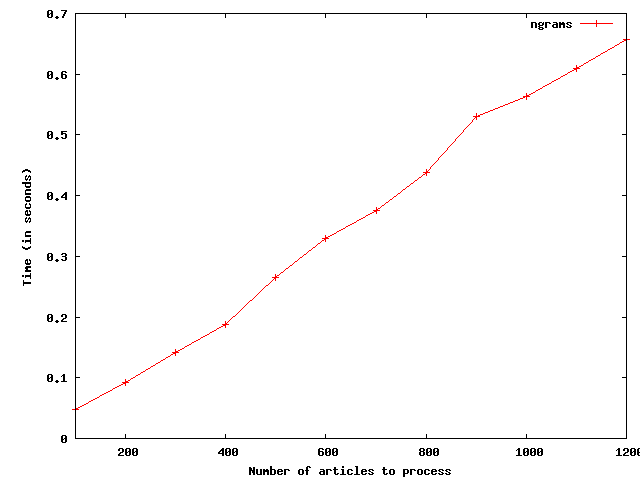
\includegraphics[width=\textwidth]{tabeller/ngram.png}\\
\caption{Time used to create $n$-grams compared to the number of texts in the corpora\label{fig:ngram}}
\end{figure}

\subsubsection{Decide authors}
The horizontal values are the number of texts in the corpora, while the vertical values are the amount of texts that have to be attributed.\\
\begin{tabular}{|c|c|c|c|c|c|c|c|c|c|c|c|c|c|}
\hline 
 & 100 & 200 & 300 & 400 & 500 & 600 & 700 & 800 & 900 & 1000 & 1100 & 1200\\ 
\hline 
100 & 55.20 & 79.24 & 100.7 & 113.7 & 127.7 & 138.9 & 152.2 & 160.5 & 170.3 & 184.5 & 193.5 & 203.4\\ 
\hline 
200 & 104.5 & 150.7 & 192.0 & 217.7 & 244.2 & 265.5 & 290.4 & 305.9 & 324.3 & 351.5 & 368.8 & 387.6\\ 
\hline 
300 & 158.7 & 229.2 & 292.7 & 330.7 & 371.3 & 403.5 & 440.8 & 464.3 & 491.9 & 533.0 & 559.0 & 587.3\\ 
\hline 
400 & 212.1 & 306.8 & 391.2 & 442.1 & 496.4 & 539.2 & 588.6 & 619.7 & 656.1 & 710.5 & 745.1 & 782.6\\ 
\hline 
500 & 279.5 & 403.9 & 514.4 & 581.0 & 652.2 & 708.1 & 772.3 & 812.6 & 860.2 & 933.9 & 981.1 & 1032\\ 
\hline 
600 & 344.3 & 497.8 & 634.8 & 717.2 & 805.7 & 874.8 & 954.2 & 1004 & 1062 & 1150 & 1206 & 1267\\ 
\hline 
700 & 385.2 & 559.0 & 713.5 & 806.1 & 905.5 & 983.0 & 1072 & 1128 & 1193 & 1292 & 1355 & 1423\\ 
\hline 
800 & 449.3 & 650.7 & 830.8 & 939.5 & 1056 & 1148 & 1253 & 1318 & 1394 & 1510 & 1583 & 1663\\ 
\hline 
900 & 521.9 & 755.8 & 965.6 & 1092 & 1228 & 1333 & 1454 & 1529 & 1618 & 1751 & 1837 & 1930\\ 
\hline 
1000 & 576.8 & 836.1 & 1068 & 1208 & 1359 & 1475 & 1619 & 1705 & 1807 & 1966 & 2069 & 2175\\ 
\hline 
1100 & 615.9 & 891.6 & 1136 & 1285 & 1541 & 1664 & 1808 & 1898 & 2004 & 2164 & 2263 & 2374\\ 
\hline 
1200 & 663.2 & 961.7 & 1227 & 1387 & 1559 & 1694 & 1848 & 1947 & 2060 & 2231 & 2340 & 2457\\ 
\hline 
\end{tabular}

Figure \ref{fig:work}, which is based on the 12th horizontal line\footnote{I have chosen this particular line, since it is the one that has to attribute all the authors, and thus would be the one that would best show if there was any significant non-linear time increase when the number of items in the corpora increased} (i.e. the bottom line in the table), clearly shows that the time required to attribute 1200 authors grows linearly with the amount of posts in the corpora.\\

Since both of these tests time consumption grows linearly with the number of texts in the corpora, its clear that the algorithm could be used in practice, given that it is able to correctly attribute the authors  

\begin{figure}[!hbp]
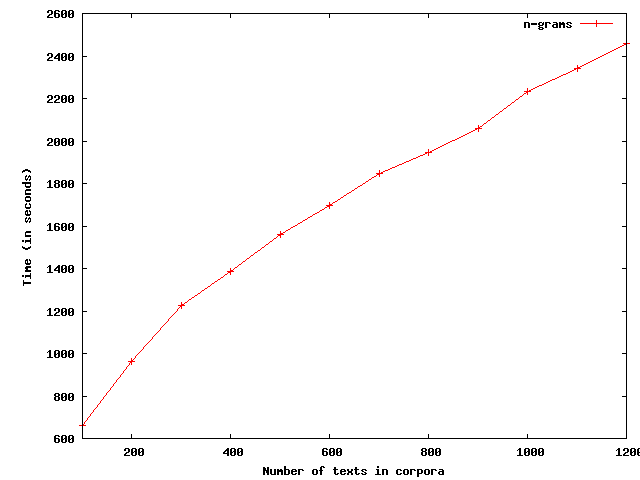
\includegraphics[width=\textwidth]{tabeller/work.png}
\caption{Time for text attribution with 1200 texts \label{fig:work}}
\end{figure}
